\documentclass[a4j]{jarticle}
    \usepackage[dvipdfmx]{graphicx}
    \usepackage[ top=25truemm,bottom=25truemm,left=25truemm,right=25truemm]
    {geometry}
    \usepackage{ascmac}
    \usepackage{array}
    \usepackage{here}
    \usepackage{here}
	\usepackage{listings, jlisting}
	\usepackage{url}
    \renewcommand{\lstlistingname}{リスト}
\lstset{language=c,
  basicstyle=\ttfamily\scriptsize,
  commentstyle=\textit,
  classoffset=1,
  keywordstyle=\bfseries,
  frame=tRBl,
  framesep=5pt,
  showstringspaces=false,
  numbers=left,
  stepnumber=1,
  numberstyle=\tiny,
  tabsize=4
}

\makeatletter
\def\@thesis{工学実験実習IV レポート}
\def\id#1{\def\@id{#1}}
\def\department#1{\def\@department{#1}}

\def\@maketitle{
\begin{center}
{\huge \@thesis \par} %修士論文と記載される部分
\vspace{10mm}
{\LARGE\bf \@title \par}% 論文のタイトル部分
\vspace{10mm}
{\Large \@date\par}	% 提出年月日部分
\vspace{20mm}
{\Large \@department \par}	% 所属部分
{\Large 学籍番号 \@id \par}	% 学籍番号部分
\vspace{10mm}
{\Large 氏名 \@author}% 氏名 
\end{center}
\par\vskip 1.5em
}

\makeatother

\title{自然言語処理}
\date{実験日1 2020年6月03日 1~2コマ目 \\ 実験日2 2020年6月10日 1~2コマ目 \\ 実験日3 2020年6月17日 1~2コマ目 \\ 実験日4 2020年6月24日 1~2コマ目 \\  実験日5 2020年7月08日 1~2コマ目 \\ 提出日 令和2年7月14日}
\department{組番号 408}
\id{17406}
\author{金澤雄大}

    \begin{document}
    \maketitle
    \thispagestyle{empty}
    \clearpage
    \addtocounter{page}{-1}

\section{目的}
自然言語処理における言語処理の基礎的な知識および開発環境を学ぶことを目的とする.
また自然言語処理の結果を分析し,文章の特徴を抽出するように改良を行うことを目的とする.
\section{理論・概要}
本章では次に示す理論,概要について述べる.
\begin{enumerate}
  \item 形態素解析
  \item Term Frequency
  \item Inverse Document Frequency
  \item Tf-Idf
\end{enumerate}
\subsection{形態素解析}
自然言語とは人間が普段話す「日本語」や「英語」を代表とする言語である.本実験では「日本語」を処理する.
例として「技術者がこの先生きのこるためにすべきことはなにか」という文について考える.
人間がこの文の意味を理解するためには,「技術者が,この先,生きのこるために,すべきことはなにか」
というように「,」で文を区切って理解するのではないだろうか.
しかし逐次的に文章をたどっていくと「技術者が,この先生,きのこるためにすべきことはなにか」という
ように解釈されることもあり得る.この解釈を一意にするため,文法の規範や辞書をもとにして,文章を形態素(単語ごとの区切り)に分割するツールが形態素解析器である.
本実験では形態素解析器としてMeCab\cite{mecab}を用いる. MeCabとは京都大学情報学研究科−日本電信電話株式会社コミュニケーション科学基
礎研究所 共同研究ユニットプロジェクトを通じて開発されたオープンソースの形態素解析エンジンである.
例えば「技術者がこの先生きのこるためにすべきことはなにか」という文章をMeCabに入力するとリスト\ref{gi}のような
出力が得られる.リスト\ref{gi}から「技術者が,この先,生きのこるために,すべきことはなにか」というように
文章を分割していることが読み取れる.また,リスト\ref{gi}のEOS(End Of Statement)は文章の終わりのことである.
\begin{lstlisting}[basicstyle=\ttfamily\footnotesize, frame=single,label=gi,caption=MeCabの出力の例]
技術	名詞,一般,*,*,*,*,技術,ギジュツ,ギジュツ
者	名詞,接尾,一般,*,*,*,者,シャ,シャ
が	助詞,格助詞,一般,*,*,*,が,ガ,ガ
この	連体詞,*,*,*,*,*,この,コノ,コノ
先	名詞,一般,*,*,*,*,先,サキ,サキ
生き	動詞,自立,*,*,一段,連用形,生きる,イキ,イキ
のこる	動詞,自立,*,*,五段・ラ行,基本形,のこる,ノコル,ノコル
ため	名詞,非自立,副詞可能,*,*,*,ため,タメ,タメ
に	助詞,格助詞,一般,*,*,*,に,ニ,ニ
す	動詞,自立,*,*,サ変・スル,文語基本形,する,ス,ス
べき	助動詞,*,*,*,文語・ベシ,体言接続,べし,ベキ,ベキ
こと	名詞,非自立,一般,*,*,*,こと,コト,コト
は	助詞,係助詞,*,*,*,*,は,ハ,ワ
なにか	副詞,助詞類接続,*,*,*,*,なにか,ナニカ,ナニカ
EOS
    \end{lstlisting}
\subsection{Term Frequency}
形態素解析の結果を用いて,文章の特徴を表すような単語を探したい.
文章の特徴を表すような単語がどのようなものであるか考えると,文書に頻繁に出現する語が文章を特徴づける
語であると考えられる.この考えを実装したものがTerm Frequency(以下tf)という重み付けである.
ある文章$d$に出てくる一つの単語$t$について,$tf$による重み${W_{tf}}_t^d$
は式(\ref{tf})で表せる.
\begin{equation}
  {W_{tf}}_t^d = \frac{tf(t,d)}{\sum_{s \in d}^{}tf(s,d)}
  \label{tf}
\end{equation}
式(\ref{tf})において$tf(t,d)$は単語$t$が文書$d$に出現する回数,$\sum_{s \in d}^{}tf(s,d)$
は文書$d$に登場する全単語数である.何故全単語数で割るかについて説明する.例として,次の2つの文書について
考える.
\begin{itemize}
  \item 全単語数200で,ある単語$t$が10回でてくる文書A.
  \item 全単語数20000で,ある単語$t$が10回でてくる文書B.
\end{itemize}
どちらもある単語$t$が10回でてくるため$tf(t,d)=10$である.しかし全単語数200であるAの方が単語$t$の登場頻度が
高いから,文書A,Bにおける単語$t$の出現頻度が同じであるという判断は正しくない.このため$tf(t,d)$を全単語数で
割る操作を行う.この操作を正規化という.

\subsection{Inverse Document Frequency}
Term Frequencyは,文書に頻繁に出現する語が文章を特徴づける語である,という考えから生まれた重みづけの方法であった.
しかし文章にまれに登場する語のほうが文章を特徴づける語なのではないか,と考えることもできる.
この考えを実装したものがInverse Document Frequency(以下idf)である.
文章にまれに登場するかどうかは他の文章と比較して決定する必要があるから,idfは複数文書間の重みづけになる.
例として,文書1万件の中で,「自動車」が含まれている文書が1000件ある場合と,「スペースシャトル」が含まれている文書が
10件ある場合では「スペースシャトル」を含む文書のほうが膨大にある文書の中から絞り込みができていると考えられる.\\
 文書の総数$N$,ある単語$t$を含んでいる文書の数を$df(t)$とする.このとき単語$t$のidf値$idf(t)$は式(\ref{idf})で表される.
\begin{equation}
  idf(t) = \log_{10} \frac{N}{df(t)} +1 
  \label{idf}
\end{equation}
単語$t$を含んでいる文書の数$df(t)$が大きくなると$\frac{N}{df(t)}$は小さくなる.
図\ref{ndf}は$N=1,10,100$のときの$\frac{N}{df(t)}$のグラフである.
\begin{figure}[H]
  \centering
  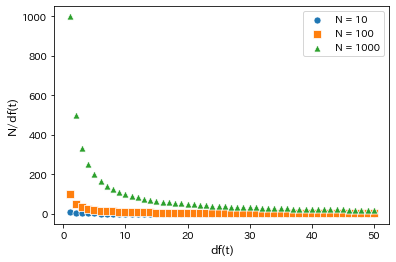
\includegraphics[scale=0.75]{ndf.png}
  \caption{$\frac{N}{df(t)}${\it vs.}$df(t)$}
 \label{ndf}
\end{figure}
図\ref{ndf}から文書数1000のとき,$\frac{N}{df(t)}$は0から1000という広い値を取ることがわかる.例として$\frac{N}{df(t)}=1000$
の単語$t_1$,$\frac{N}{df(t)}=10$の単語$t_2$,$\frac{N}{df(t)}=1$の単語$t_3$の3単語があったとする.
3単語を比較したときに単語$t_1$は単語$t_2$よりどれぐらい文書を特徴付ける単語なのか,単語$t_2$は単語$t_3$よりどれぐらい文書を特徴付ける単語なのか
が分かりにくい.このため$\frac{N}{df(t)}$に対数変換を行って$idf(t)$が右に裾の長い分布になることを抑える必要がある.
図\ref{idfpic}は$N=1,10,100$のときの$idf(t)$のグラフである.
図\ref{idfpic}では対数変換によって重みづけ$idf(t)$が滑らかになっており,単語の$idf(t)$を相対的に
比較したときに,どちらがより文書の特徴を表す語であるかがわかりやすい.
\begin{figure}[H]
  \centering
  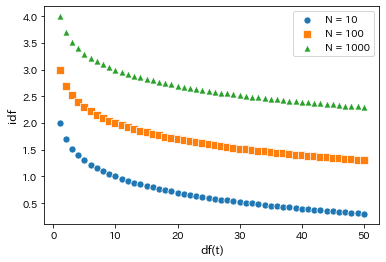
\includegraphics[scale=0.75]{idf.png}
  \caption{$idf(t)${\it vs.}$df(t)$}
 \label{idfpic}
\end{figure}
\subsection{Tf-Idf}
文書に出現する頻度の高さを特徴として表す重みづけとしてTerm Frequencyを与え,文書群での出現頻度が
低い,稀である特徴を表す重みづけとしてInverse Document Frequencyを与えた.Term Frequencyは文書から
導出した値で,Inverse Document Frequencyは文書群から導出した値であるので,互いの値を組み合わせて,文書群に
含まれる文書の特徴の重みづけとしてTerm Frequency-Inverse Document Frequency(Tf-Idf)を与える.これによって
文書中の出現品後が少ない単語でも,他の文書に含まれていない場合は,この文書を特徴づける重みとして,有効に
作用すると予想される.\\
式\ref{tfidf}は文書dに登場する単語tにおけるTf-Idfの重み${W_{tf-idf}}_t^d$を表している.
\begin{equation}
  {W_{tf-idf}}_t^d = \frac{tf(t,d)}{\sum_{s \in d}^{}tf(s,d)} \times \left( \log_{10} \frac{N}{df(t)} +1 \right)
  \label{tfidf}
\end{equation}


\section{実験方法}
本章では開発環境および実験手順について述べる.
\subsection{開発環境}
開発環境を表\ref{kankyou}に示す.授業中の資料では文字コードはSJISを用いることになっているが
他環境と競合するためUTF-8を用いる.
\begin{table}[H]
  \caption{開発環境}
  \label{kankyou}
  \begin{center}
      \begin{tabular}{l|c}\hline
        CPU & Intel Core i7-6500 2.50Ghz \\ 
        メモリ & 16.0GB DDR3 \\
        OS & Windows 10 Home \\
        統合開発環境 & Eclipse Java EE IDE for Web Developers. Version: 2018-09 (4.9.0)\\
        開発言語 & Java 08 \\
        文字コード & UTF-8 \\ \hline
      \end{tabular}
  \end{center}
  \end{table}

\subsection{実験手順}
本実験では,001.txtから100.txtまでの100文書を用いて実験を行う.実験や解析に用いる文書全体をコーパスと呼ぶ.
本実験ではコーパスをdata-utf8ディレクトリ下に置いている.
本実験で扱う文書の例として,付録のリスト\ref{001all}に001.txtの全文を示す.
リスト\ref{001all}から文書ファイルの中身は文章のみで構成されていることがわかる.
他の文書ファイルも同様の形式になっている.
	
次に示す手順で実験を行う.各重みを計算し,計算結果をtxtファイルに書き出すプログラムを実装する.
ただし,本レポートではMeCabの環境構築,およびEclipseの使用方法については
説明しない.
\begin{enumerate}
  \item 形態素解析とTerm Frequencyの実装
  \item Inverse Document Frequencyの実装
  \item Term Frequency-Inverse Document Frequencyの実装
  \item 実行結果の分析と改良
\end{enumerate}

\section{Term Freqencyの実装と実行結果}
本章ではTerm Freqencyの実装と実行結果について述べる.
\subsection{プログラムの説明}
Term Frequencyの実装は次の6つのクラスを作成して行う.本節ではこの6つのクラスの説明について述べる.
\begin{enumerate}
  \item Wordクラス
  \item WordCountクラス
  \item TfCountクラス
  \item WordCompareクラス
  \item TermFrequencyクラス
  \item NaturalLanguageProcessingクラス(メイン)
\end{enumerate}

\subsubsection{Wordクラス}
リスト\ref{gi}に示したように,MeCabの実行結果は分割した品詞の種類,活用形を代表とする多数の情報を
出力する.表\ref{mecabout}はMecabの実行時に出力される情報と「渡し」のときの例である.
\begin{table}[H]
  \caption{Mecabの出力情報}
  \label{mecabout}
  \begin{center}
      \begin{tabular}{l|l}\hline
        素性情報 & 「渡し」の例 \\ \hline
        \hline
        表層系 & 渡し \\
        品詞 & 動詞 \\
        品詞細分類1 & 自立 \\ 
        品詞細分類2 & * \\ 
        品詞細分類3 & * \\ 
        活用型 & 五段・サ行\\
        活用形 & 連用形 \\
        基本形 & 渡す \\
        読み & ワタシ \\
        発音 & ワタシ \\ \hline
      \end{tabular}
  \end{center}
  \end{table}
  MeCabから出力される素性情報を格納するクラスとしてWordクラスを作成する.リスト\ref{WordClass}にWordクラスのソースコードを示す.
  ただし,フィールド変数のセッターおよびゲッターは省略する.
  Wordクラスはフィールドにprivate変数として表\ref{mecabout}の出力結果を持つ.また,メソッドとしてセッター,およびゲッター,および
  2つの変数の一致/不一致をbooleanで出力するequalsメソッドを設ける.フィールド変数をprivateとして,セッターおよびゲッターを設けるのは
  外部からの入力で変数を不正な値にされることを防ぐためである.オブジェクト指向において,クラス内のフィールドおよびメソッドを
  外部から保護することをカプセル化という.
  \begin{lstlisting}[basicstyle=\ttfamily\footnotesize, frame=single,label=WordClass,caption=Wordクラスのソースコード]
package nlp;

class Word
{

	// セッターおよびゲッターは省略

	public boolean equals(Object obj)
	 {
	 //オブジェクトが null の場合,不一致
	 if(obj == null)
	 {
	 return false;
	 }
	 //オブジェクトの型が異なる場合,不一致
	 if(!(obj instanceof Word))
	 {
	 return false;
	 }
	 //オブジェクトの全てのフィールドが一致している場合,一致
	 if(
	 ((((Word)obj).getHyousoukei() == null && this.getHyousoukei() == null)
	 ||((Word)obj).getHyousoukei().equals(this.getHyousoukei()))
	 && ( (((Word)obj).getHinshi() == null && this.getHinshi() == null)
	 ||((Word)obj).getHinshi().equals(this.getHinshi()))
	 && ( (((Word)obj).getHinshi1() == null && this.getHinshi1() == null)
	 ||((Word)obj).getHinshi1().equals(this.getHinshi1()))
	 && ( (((Word)obj).getHinshi2() == null && this.getHinshi2() == null)
	 ||((Word)obj).getHinshi2().equals(this.getHinshi2()))
	 && ( (((Word)obj).getHinshi3() == null && this.getHinshi3() == null)
	 ||((Word)obj).getHinshi3().equals(this.getHinshi3()))
	 && ( (((Word)obj).getKatsuyoKata() == null && this.getKatsuyoKata() == null)
	 ||((Word)obj).getKatsuyoKata().equals(this.getKatsuyoKata()))
	 && ( (((Word)obj).getKatsuyoKei() == null && this.getKatsuyoKei() == null)
	 ||((Word)obj).getKatsuyoKei().equals(this.getKatsuyoKei()))
	 && ( (((Word)obj).getGenkei() == null && this.getGenkei() == null)
	 ||((Word)obj).getGenkei().equals(this.getGenkei()))
	 && ( (((Word)obj).getYomi() == null && this.getYomi() == null)
	 || ((Word)obj).getYomi().equals(this.getYomi()))
	 && ( (((Word)obj).getHatsuon() == null && this.getHatsuon() == null)
	 || ((Word)obj).getHatsuon().equals(this.getHatsuon()))
	 )
	 {
	 return true;
	 }
	 //そのほかは不一致
	 return false;
	 }

 private String hyousoukei = null;//表層形
 private String hinshi = null;//品詞
 private String hinshi1 = null;//品詞細分類 1
 private String hinshi2 = null;//品詞細分類 2
 private String hinshi3 = null;//品詞細分類 3
 private String katsuyoKata = null;//活用型
 private String katsuyoKei = null;//活用形
 private String genkei = null;//原形
 private String yomi = null;//読み
 private String hatsuon = null;//発音

}
    \end{lstlisting}
    
\subsubsection{WordCountクラス}
tf値を計算する際に単語の出現回数の情報が必要であるから,これを記憶するWordCountクラスを作成する.
WordCountクラスはフィールドにprivate変数としてWord型の変数wordと,
単語の出現回数を保持するInteger型の変数countを設ける.
また,メソッドとしてコンストラクタ,およびフィールド変数のセッター,およびゲッターを設ける.
WordCountクラスのソースコードは省略する.


\subsubsection{TfCountクラス}
tfの計算結果を保持するクラスとして,WordCountクラスを継承して,TfCountクラスを作成する.
TfCountクラスのフィールドにはtfの計算結果を保持する変数として,private Double型の変数tfを設ける.
またメソッドとして,コンストラクタ,および変数tfのセッターおよびゲッターを設ける.
TfCountクラスのソースコードは省略する.

\subsubsection{WordCompareクラス}
tfの計算結果を出力するときに,tf値で結果をソートしてファイル出力を行う.
このため,2つのWordCount型変数の出現回数を大小比較するクラスとしてWordCompareクラスを作成する.リスト\ref{WordCompareClass}にWordCompareクラスのソースコードを示す.
WordCompareクラスはComparatorインターフェースを実装している.compare関数の仕様はJava APIドキュメント\cite{javaapi}にあるように2つのオブジェクトo1,o2を引数として,
最初の引数o1が2番目の引数o2より小さい場合は負の整数(-1)、両方が等しい場合は0、最初の引数o1が2番目の引数o2より大きい場合は正の整数(1)を返す.
\begin{lstlisting}[basicstyle=\ttfamily\footnotesize, frame=single,label=WordCompareClass,caption=WordCompareクラスのソースコード]
package nlp;

import java.util.Comparator;

class WordCompare implements Comparator<WordCount>
{
 @Override
 public int compare(WordCount wc1, WordCount wc2)
 {
 if(wc1.getCount() < wc2.getCount())
 return 1;
 if(wc1.getCount() == wc2.getCount())
 return 0;
 if(wc1.getCount() > wc2.getCount())
 return -1;
 return 0;
 }
}
    \end{lstlisting}

    \subsubsection{TermFrequencyクラス}
    1つのファイルについて形態素解析およびtfの計算を行い,ファイルに書き込む関数としてTermFrequencyクラスを実装する.
    リスト\ref{TermFrequencyClass}にTermFrequencyクラスのソースコードを示す.TermFrequencyクラスはフィールドにTfCount型のリストlistを持つ.
    またtfメソッドを持つ.tfメソッドの引数,および返り値,および処理内容を表\ref{tfc}に示す.
    \begin{lstlisting}[basicstyle=\ttfamily\footnotesize, frame=single,label=TermFrequencyClass,caption=TermFrequencyクラスのソースコード]
package nlp;

import java.io.BufferedReader;
import java.io.FileWriter;
import java.io.IOException;
import java.io.InputStreamReader;
import java.util.ArrayList;

public class TermFrequency {

	ArrayList<TfCount> list = new ArrayList<TfCount>();

	public void tf(String inputFilename, String outputFilename){

		//String inputFilename = "data-utf8\\001.txt";
		String[] command = {"cmd.exe", "/C", "mecab", inputFilename };

		 try {
			 Process ps = Runtime.getRuntime().exec(command);
			 BufferedReader bReader_i = new BufferedReader(
         new InputStreamReader(ps.getInputStream(), "UTF-8"));
			 String targetLine;

			 while (true) {
				 targetLine = bReader_i.readLine();

				 if (targetLine == null) {
					 break;
				 }
				 else if (targetLine.equals("EOS")) {
					 continue;
				 }
				 else {
					 Word wo = new Word();
					 String targetArray[] = targetLine.split("[\t|,]");

					 if (targetArray.length >= 1)
						 wo.setHyousoukei(targetArray[0]);
					 if (targetArray.length >= 2)
						 wo.setHinshi(targetArray[1]);
					 if (targetArray.length >= 3)
						 wo.setHinshi1(targetArray[2]);
					 if (targetArray.length >= 4)
						 wo.setHinshi2(targetArray[3]);
					 if (targetArray.length >= 5)
						 wo.setHinshi3(targetArray[4]);
					 if (targetArray.length >= 6)
						 wo.setKatsuyoKata(targetArray[5]);
					 if (targetArray.length >= 7)
						 wo.setKatsuyoKei(targetArray[6]);
					 if (targetArray.length >= 8)
						 wo.setGenkei(targetArray[7]);
					 if (targetArray.length >= 9)
						 wo.setYomi(targetArray[8]);
					 if (targetArray.length >= 10)
						 wo.setHatsuon(targetArray[9]);

					//リストの中に同じ語のエントリがあるか調べて,既にエントリがあれば,カウントアップする
					 int i;
					 for (i = 0; i < list.size(); i++) {
						 if (list.get(i).getWord().equals(wo))     {
							 list.get(i).setCount(list.get(i).getCount() +1);
							 break;
						 }
					 }
					 //リストにエントリが無かったときは,新しい語としてリストに追加する
					 if (i == list.size()) {
						 list.add(new TfCount(wo, Integer.valueOf(1)));
					 }

					 //System.out.println(targetLine);
				 }
			 }

		 }
		 catch (IOException e) {
			 e.printStackTrace();
		 }

		//今のリストのエントリをすべて表示する
		 int sum = 0;
		 for (int i = 0; i < list.size(); i++){
       //System.out.println(list.get(i).getWord()
       .getHyousoukei()+ ":" + list.get(i).getCount());
			 sum += list.get(i).getCount();
		 }

		 list.sort(new WordCompare());

		 try {
			 //String outputFilename = "data-utf8\\001tf.txt";
			 FileWriter fw = new FileWriter(outputFilename);
			 //System.out.println(outputFilename);
			 for (int i = 0; i < list.size(); i++){
				 //System.out.println(fileal.get(i).word.getHyousoukei() + 
				 ":"+ fileal.get(i).getCount());
				 list.get(i).setTf((double) list.get(i).getCount() / (double) sum);

				 fw.write(list.get(i).getWord().getHyousoukei() + "\t"
						 + list.get(i).getWord().getHinshi() + "\t"
						 + list.get(i).getWord().getHinshi1() + "\t"
						 + list.get(i).getCount() + "\t"
						 + String.format("%.10f", list.get(i).getTf()) + "\n");
			 }
			 fw.close();
		 }
		 catch (IOException ex) {
			ex.printStackTrace();
		 }

	}
}
          \end{lstlisting}

\begin{table}[H]
  \caption{tfメソッドの概要}
  \label{tfc}
  \begin{center}
      \begin{tabular}{l|l}\hline
        引数 & 入力ファイル名,出力ファイル名 \\ 
        返り値 & void \\ 
        処理内容 & 入力ファイルの形態素解析およびtfの計算を行い,出力ファイルに書き出す. \\ \hline
      \end{tabular}
  \end{center}
  \end{table}

  tfメソッドの処理内容の詳細は次の通りである.
  \begin{enumerate}
    \item 入力ファイルについて形態素解析を行う.
    \item 形態素解析の結果を1行づつ読み込み,形態素解析の結果をリストlistに書き込み,単語の出現回数をカウントする.
    \item 形態素解析の結果がEOSに辿り着いたとき,リストへの書き込みと単語の出現回数カウントを終了する.
    \item リストlistを単語の出現回数で降順にソートする.
    \item 必要であれば,リストに含まれている単語を標準出力する.
    \item 出力ファイルにリストlistの内容(表層系,品詞,出現回数,tf値)を書き出す.区切りはタブとする.
  \end{enumerate}

\subsubsection{NaturalLanguageProcessingクラス(メイン)}
メインクラスとしてNaturalLanguageProcessingクラスを作成する.メインクラスの役割は100件の文書ファイルについてTermFrequencyクラスを
インスタンス化し,tfメソッドを実行することである.リスト\ref{NaturalLanguageProcessingClass1}にNaturalLanguageProcessingクラスのソースコードを示す.
main関数では長さ100のtfクラスの配列を用意し,for文を用いて各文書の解析情報を格納するtf配列の要素をインスタンス化し,tfメソッドの実行をしている.
\begin{lstlisting}[basicstyle=\ttfamily\footnotesize, frame=single,label=NaturalLanguageProcessingClass1,caption=NaturalLanguageProcessingクラスのソースコード]
package nlp;
public class NaturalLanguageProcessing
{
 static public void main(String args[])
 {
 System.out.println("TF calculate");
 TermFrequency[] tf= new TermFrequency[100];
 for(int i=1; i <= 100;i++)
 {
 tf[i-1] = new TermFrequency();
 String inputFileName = "data-utf8\\" + String.format("%03d", i) + ".txt";
 String outputFileName = "data-utf8\\" + String.format("%03d", i) + "tf.txt";
 //System.out.println(inputFileName);
 System.out.println(outputFileName);
 tf[i-1].tf(inputFileName,outputFileName);
 }
 System.out.println("complete");
 }
}

\end{lstlisting}

\subsection{実行結果}
本節では実行結果として,標準出力および形態素解析とtfの計算結果について述べる.
\subsubsection{標準出力}
リスト\ref{NaturalLanguageProcessingClass1}に示したように,NaturalLanguageProcessingクラスでは書き込み先ファイルと,実行終了時に"complete"の文字列を
表示する.図\ref{starttf}および図\ref{endtf}は,プログラム実行時の標準出力を示している.図\ref{starttf}から001.txtから順に形態素解析およびtfの計算を
行い,図\ref{endtf}から100.txtまで同様の処理を行って実行を終了したことがわかる.
これより標準出力において,エラーや予期しない挙動が起きることなく処理が行えていることが分かる.
\begin{figure}[H]
	\centering
	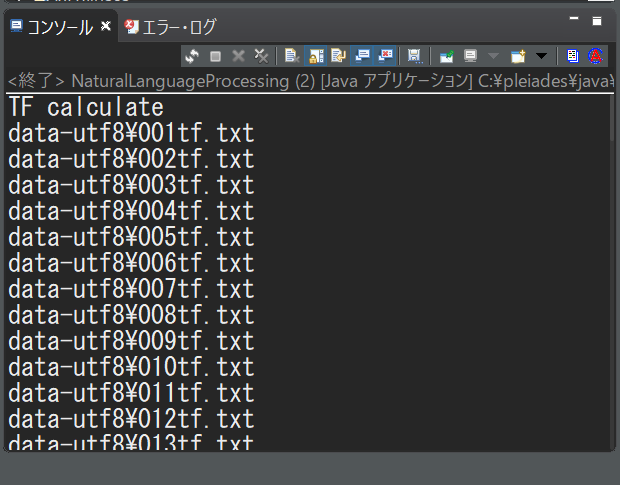
\includegraphics[scale=0.65]{starttf.png}
	\caption{プログラム実行開始時の標準出力}
   \label{starttf}
  \end{figure}

  \begin{figure}[H]
	\centering
	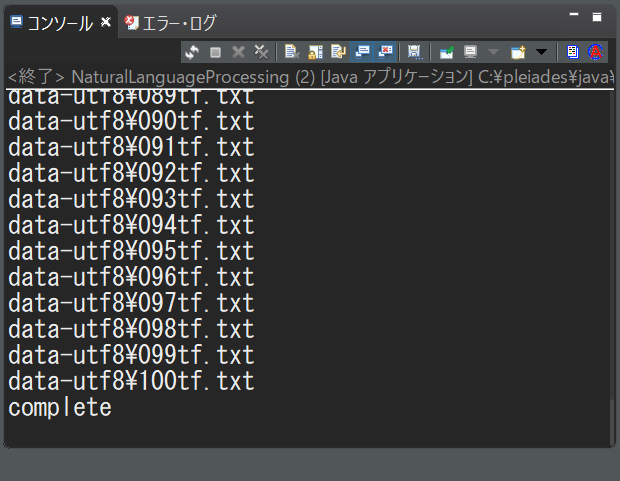
\includegraphics[scale=0.65]{endtf.png}
	\caption{プログラム実行終了時の標準出力}
   \label{endtf}
  \end{figure}

\subsubsection{形態素解析とtf値の計算結果}
形態素解析の結果は001tf.txtから100tf.txtに書き込まれている.例として,リスト\ref{001tf}に001.txtのプログラム実行結果
を示す.また,リスト\ref{002tf}に002.txtの実行結果を示す.リスト\ref{001tf}およびリスト\ref{002tf}から表層系,品詞,出現回数,tf値が書き込まれていることがわかる.
また文書によって実行結果が異なっていることが読み取れる.
\begin{lstlisting}[basicstyle=\ttfamily\footnotesize, frame=single,label=001tf,caption=001tf.txtの抜粋]
%	名詞	41	0.0764925373
天然記念物	名詞	16	0.0298507463
E	名詞	16	0.0298507463
の	助詞	13	0.0242537313
地	名詞	13	0.0242537313
〔	記号	11	0.0205223881
県	名詞	11	0.0205223881
〕	記号	11	0.0205223881
(	記号	10	0.0186567164
)	記号	10	0.0186567164
	\end{lstlisting}

\begin{lstlisting}[basicstyle=\ttfamily\footnotesize, frame=single,label=002tf,caption=002tf.txtの抜粋]
学,名詞,44,0.0449438202
、,記号,40,0.0408580184
人類,名詞,38,0.0388151175
経済,名詞,35,0.0357507661
の,助詞,34,0.0347293156
・,記号,26,0.0265577120
。,記号,21,0.0214504597
 ,記号,19,0.0194075587
は,助詞,17,0.0173646578
を,助詞,16,0.0163432074
	\end{lstlisting}

出現回数,tf値の計算が正しく行われていることを確認する.「天然記念物」という単語に着目する.付録のリスト\ref{001all}から001.txt
は「天然記念物」が16回登場するとわかる.リスト\ref{001tf}における「天然記念物」の出現回数は16になっているから
出現回数のカウントは正しく行われていることがわかる.また,excelを代表とするツールを用いると出現回数の総和,つまり全単語数Nは536であることが
わかる.これよりtf値は$\frac{16}{536}=0.0298\dots$と計算できる.リスト\ref{001tf}における「天然記念物」のtf値は0.0298507463になっているから
tf値の計算も正しく行われていることが確認できた.\\
 次に,tf値が正規化によって文字数の量に依存しない値になっていることを確認する.tf値が正規化によって文字数の量に依存しない値になっていることは
同じ単語が同じ回数登場する2つの文章の全単語数とtf値を比較することで確認できる.ここでは001.txtと002.txtを用いる.
表\ref{tfh}は001.txtおよび002.txtにおける全単語数,および「出典」の出現回数,およびtf値を
示したものである.
\begin{table}[H]
	\caption{001.txtと002.txtの全単語数,「出典」の出現回数とtf値}
	\label{tfh}
	\begin{center}
		\begin{tabular}{c|c c}\hline
			項目 & 001.txt & 002.txt \\ \hline
			\hline
			全単語数 & 536 & 979 \\ 
			「出典」の出現回数 & 1 & 1 \\
			「出典」のtf値 & 0.0018656716 & 0.0010214505 \\ \hline
 		\end{tabular}
	\end{center}
	\end{table}

	表\ref{tfh}から001.txtおよび002.txtにおける「出典」の出現回数はどちらも1である.しかし,002.txtの全単語数は001.txtのおよそ2倍であるから,
	tf値が正規化によって文字数の量に依存しない値であれば,002.txtにおける「出典」のtf値は001.txtにおける「出典」のtf値の$\frac{1}{2}$であることが予想される.
	表\ref{tfh}から,002.txtにおける「出典」のtf値は0.0010214505で,001.txtにおける「出典」のtf値は0.0018656716であるから,
	001.txtにおける「出典」のtf値が002.txtにおける「出典」のtf値の1.8倍であることが計算できる.これより,tf値が正規化によって文字数の量に依存しない値
	であることが確認できた.

\section{Inverse Document Frequencyの実装と実行結果}
本章ではInverse Document Frequencyの実装と実行結果について述べる.
\subsection{プログラムの説明}
Inverse Document Frequencyの実装は次の3つのクラスを作成,追記して行う.本節ではこの3つのクラスの説明について述べる.
\begin{enumerate}
  \item DfCountクラス
  \item DocumentFrequencyクラス
  \item NaturalLanguageProcessingクラス(メイン)
\end{enumerate}

\subsubsection{DfCountクラス}
計算したidf値を保持するクラスとして,Term Frequencyの実装で作成したWordCountクラスを継承して,
DfCountクラスを作成する.
DfCountクラスはフィールドにidf値を保持するprivate Double型の変数idfを
持つ.またメソッドとしてコンストラクタ,およびidfのセッター,ゲッターを設ける.
DfCountクラスのソースコードは省略する.

\subsubsection{DocumentFrequencyクラス}
100件の文書のidfを計算するクラスとしてDocumentFrequencyクラスを作成する.
リスト\ref{DocumentFrequencyClass}にDocumentFrequencyクラスのソースコードのソースコードを示す.
DocumentFrequencyクラスではフィールドにDfCount型のリストlist,
およびTermFrequency型の配列(TermFrequencyの実行結果のリスト)を持つ.
また,メソッドとしてコンストラクタおよび,dfメソッドを持つ.
\begin{lstlisting}[basicstyle=\ttfamily\footnotesize, frame=single,label=DocumentFrequencyClass,caption=DocumentFrequencyクラスのソースコード]
package nlp;

import java.io.FileWriter;
import java.io.IOException;
import java.util.ArrayList;

public class DocumentFrequency
{
 //DF をカウントするためのデータ格納領域の定義
 ArrayList<DfCount> list = new ArrayList<DfCount>();
 //DF の元になる TF を受ける
 TermFrequency tf[];
 DocumentFrequency(TermFrequency[] tf)
 {
 this.tf = tf;
 }
 public void df(String outputFilename)
 {
 //(ここに処理を定義する)
 //TF100 ファイル分について繰り返す
 for(int i=1;i<=100;i++) {
	 System.out.println("df calculate : "+String.format("%03d", i));
	//TF1 件に含まれる語の分だけ繰り返し
	 for(int j=0;j<tf[i-1].list.size();j++) {
		 //DF のリストの中にエントリがあるか調べる
		//System.out.rintln(tf[i-1].list.get(j)
		.getWord().getHyousoukei());
		 int k;
		 for(k=0;k<list.size();k++) {
		 if(list.get(k).getWord().equals(tf[i-1].list.get(j).getWord())) {
			 list.get(k).setCount(list.get(k).getCount() +1);
			 break;
		 }
		 }
		 //リストにエントリが無かったときは,新しい語としてリストに追加する
		 if (k == list.size()) {
			 list.add(new DfCount(tf[i-1].list.get(j)
			 .getWord(), Integer.valueOf(1)));
		 }
	 }
	 }
 //ソートする
 list.sort(new WordCompare());

 //今のリストのエントリをすべて表示する
 for (int i = 0; i < list.size(); i++){
	 //System.out.println(list.get(i).getWord()
	 .getHyousoukei()+ ":" + list.get(i).getCount());
 }

 //df,idf の結果をファイルに保存する
 try {
	 FileWriter fw = new FileWriter(outputFilename);
	 //System.out.println(outputFilename);
	 for (int i = 0; i < list.size(); i++){
		 //System.out.println(fileal.get(i).word
		 .getHyousoukei() + ":"+ fileal.get(i).getCount());
		 list.get(i).setIdf(Math.log10((double) 100 / 
		 (double) list.get(i).getCount())+1);

		 fw.write(list.get(i).getWord().getHyousoukei() + "\t"
				 + list.get(i).getCount() + "\t"
				 + list.get(i).getWord().getHinshi() + "\t"
				 + String.format("%.10f", list.get(i).getIdf()) + "\n");
	 }
	 fw.close();
 }
 catch (IOException ex) {
	ex.printStackTrace();
 }
 }
}
\end{lstlisting}
 コンストラクタでは,文書100件分の形態素解析およびTermFrequencyの計算結果を保持するTermFrequency
型の配列tfをフィールドのtfに受け取る処理を行う.\\
dfメソッドはtfを用いてdf,idfを計算する処理を行う.dfメソッドは引数として出力ファイル(String型)
を受け取る.返り値はvoid型である.
dfメソッドの処理内容の詳細は次の通りである.
\begin{enumerate}
	\item 1件の文書について,1つの単語に着目し,その単語がリストdfに含まれていれば
	カウントをインクリメントする.リストdfに含まれていない場合はリストに追加しカウントを0にする.
	\item 1件の文書について,すべての単語で同様の処理を行う.
	\item 100件の文書すべてで同様の処理を行う. 
	\item リストdfをidf値の降順にソートする.
	\item 必要があればリストの内容を表示する.
	\item 式(\ref{idf})を用いてリストdfのすべての単語についてidf値を計算する.
	\item リストdfの全ての単語について,表層系,および出現回数,および品詞,およびidf値を出力ファイルに書き込む.
	\item ファイルを閉じて処理を終了する.
\end{enumerate}

\subsubsection{NaturalLanguageProcessingクラス(メイン)}
tfの計算時に作成したメインクラスにidfの計算の実行を追記する.
リスト\ref{NaturalLanguageProcessingClass2}にNaturalLanguageProcessingクラスのソースコードの追記部分を示す.
形態素解析とtfの計算の後に,dfクラスとインスタンス化し,dfメソッドを実行する処理を追記した.
\begin{lstlisting}[basicstyle=\ttfamily\footnotesize, frame=single,label=NaturalLanguageProcessingClass2,caption=NaturalLanguageProcessingクラスのソースコード(追記部分)]
System.out.println("DF calculate");
DocumentFrequency df = new DocumentFrequency(tf);
String outputFilename = "data-utf8\\df.txt";
df.df(outputFilename);
	\end{lstlisting}
\subsection{実行結果}
本節では実行結果として, 標準出力およびidf値の計算結果について述べる.
\subsubsection{標準出力}
NaturalLanguageProcessingクラスおよびDocumentFrequencyクラスでは
処理を行っている文書の番号と,実行終了時に"complete"の文字列を表示する.
図\ref{startidf}および図\ref{endidf}にidfの計算実行時の標準出力を示す.
図\ref{startidf}からtf値の計算終了後に文書001から順にidf値の計算が行われていることがわかる.
また,図\ref{endidf}から文書100までidf値を計算し,最後に"complete"の文字列を表示して処理を終了している.
これより標準出力において,エラーや予期しない挙動が起きることなく処理が行えていることが分かる.
\begin{figure}[H]
	\centering
	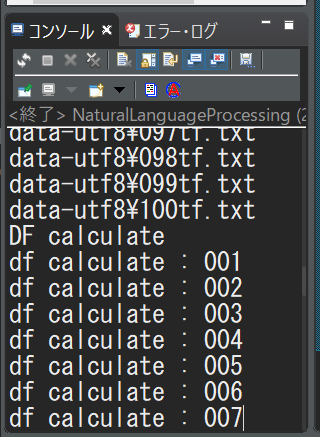
\includegraphics[scale=0.65]{idfstart.png}
	\caption{idfの計算実行時の標準出力1}
   \label{startidf}
  \end{figure}

\begin{figure}[H]
	\centering
	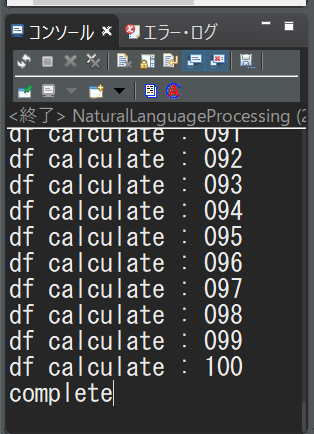
\includegraphics[scale=0.65]{idfend.png}
	\caption{idfの計算実行時の標準出力2}
   \label{endidf}
  \end{figure}

\subsubsection{idf値の計算結果}
idfの計算結果はdf.txtに書き込まれている.
リスト\ref{dfhead}にdf.txtの冒頭10行を示す.また,リスト\ref{dftail}にdf.txtの末尾10行を示す.
どちらのリストにおいても表層系,df値,品詞,idf値の順になっている.
リスト\ref{dfhead}から冒頭10行のdf値が全て100になっており,idf値もすべて1.0になっていることがわかる.
またリスト\ref{dftail}から末尾10行のdf値が全て1になっており,idf値もすべて3.0になっていることがわかる.
先頭および末尾の10行を見ただけではidf値の計算結果が正しいかわからない.
\begin{lstlisting}[basicstyle=\ttfamily\footnotesize, frame=single,label=dfhead,caption=df.txtの冒頭10行]
の	100	助詞	1.0000000000
(	100	記号	1.0000000000
)	100	記号	1.0000000000
、	100	記号	1.0000000000
。	100	記号	1.0000000000
.	100	名詞	1.0000000000
:	100	名詞	1.0000000000
は	100	助詞	1.0000000000
を	100	助詞	1.0000000000
に	100	助詞	1.0000000000
\end{lstlisting}

\begin{lstlisting}[basicstyle=\ttfamily\footnotesize, frame=single,label=dftail,caption=df.txtの末尾10行]
いたずら	1	名詞	3.0000000000
ハイアワサ	1	名詞	3.0000000000
風車	1	名詞	3.0000000000
シンフォニー	1	名詞	3.0000000000
消防	1	名詞	3.0000000000
子ども	1	名詞	3.0000000000
交響楽	1	名詞	3.0000000000
人魚	1	名詞	3.0000000000
ハリウッド	1	名詞	3.0000000000
マザーグース	1	名詞	3.0000000000
働き	1	動詞	3.0000000000
\end{lstlisting}

サクラエディタのgrep検索機能を用いてidf値の計算結果が正しいか確認する.
ここでは「日本人」という単語に着目する.df.txtにおける「日本人」のidf値の計算結果は
「日本人	6	名詞	2.2218487496」になっている.図\ref{japanese}はサクラエディタのgrep検索機能で
tf値の出力結果(001tf.txt~100tf.txt)のうち「日本人」を含む文書を検索した結果である.
図\ref{japanese}から「日本人」を含む文書は6つあることがわかる.これはdf.txtの「日本人」のdf値と
一致している.また式(\ref{idf})を用いて「日本人」のidf値を計算すると2.2218487496であることが
わかる.これよりdf値,idf値の計算が正しいことが確かめられた.
\begin{figure}[H]
	\centering
	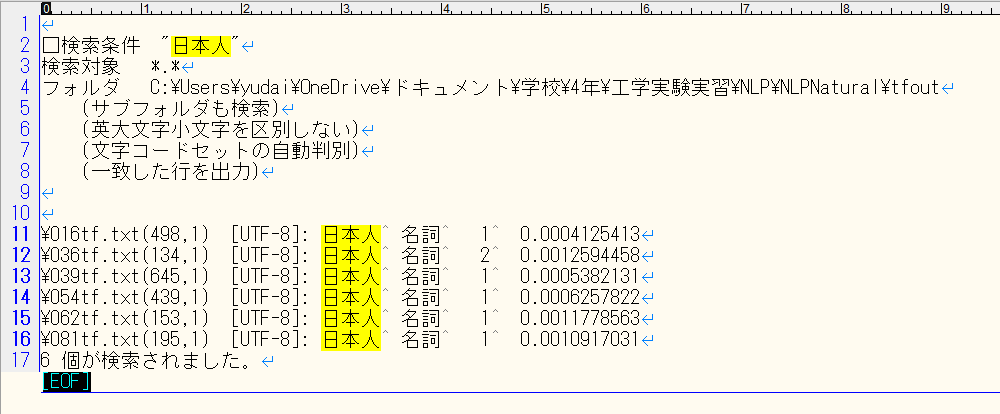
\includegraphics[scale=0.75]{japanese.png}
	\caption{「日本人」が出現する文書}
   \label{japanese}
  \end{figure}

\section{Term Frequency-Inverse Document Frequencyの実装と実行結果}
本章ではTerm Frequency-Inverse Document Frequencyの実装と実行結果について述べる.
\subsection{プログラムの説明}
Term Frequency-Inverse Document Frequencyの実装は次の4つのクラスを作成,追記して行う.本節ではこの4つのクラスの説明について述べる.
\begin{enumerate}
  \item TfIdfCountクラス
  \item TfIdfcompareクラス
  \item TfIdfクラス
  \item NaturalLanguageProcessingクラス(メイン)
\end{enumerate}

\subsubsection{TfIdfCountクラス}
idf値およびtfidf値を保持するクラスとして,TfCountクラスを継承したTfIdfCountクラスを作成する.
TfIdfCountクラスはフィールドとして,Double型変数のtfidf,idfを持つ.
またメソッドとしてコンストラクタおよびフィールド変数のセッター,およびゲッターを設ける.
TfIdfCountクラスのソースコードは省略する.

\subsubsection{TfIdfcompareクラス}
計算したtfidf値でリストをソートするために,TfIdfcompareクラスを作成する.
リスト\ref{TfIdfcompareClass}にTfIdfcompareクラスのソースコードを示す.
TfIdfcompareクラスはTfIdfCount型のComparatorを実装している.Comparatorの実装については
WordCompareクラスの説明で行ったため,ここでは省略する.
\begin{lstlisting}[basicstyle=\ttfamily\footnotesize, frame=single,label=TfIdfcompareClass,caption=TfIdfcompareクラスのソースコード]
package nlp;

import java.util.Comparator;

public class TfIdfcompare implements Comparator<TfIdfCount>{
	@Override
	 public int compare(TfIdfCount wc1, TfIdfCount wc2)
	 {
	 if(wc1.getTfidf() < wc2.getTfidf())
	 return 1;
	 if(wc1.getTfidf() == wc2.getTfidf())
	 return 0;
	 if(wc1.getTfidf() > wc2.getTfidf())
	 return -1;
	 return 0;
	 }
}
	\end{lstlisting}

\subsubsection{TfIdfクラス}
文書100件分のtfidfを計算するクラスとしてTfIdfクラスを作成する.
リスト\ref{TfIdfClass}にTfIdfクラスのソースコードを示す.
TfIdfクラスはフィールドにTfIdfカウント型のリストlist,およびtf,idfの計算結果であるtfの配列とdfを持つ.
またメソッドとしてコンストラクタとtfidfメソッドを持つ.
\begin{lstlisting}[basicstyle=\ttfamily\footnotesize, frame=single,label=TfIdfClass,caption=TfIdfクラスのソースコード]
package nlp;

import java.io.FileWriter;
import java.io.IOException;
import java.util.ArrayList;

public class TfIdf {

	ArrayList<TfIdfCount> list = new ArrayList<TfIdfCount>();
	TermFrequency[] tf;
	DocumentFrequency df;
	TfIdf(TermFrequency[] tf,DocumentFrequency df){
		this.tf = tf;
		this.df = df;
	}

	public void tfidf() {
		for(int i=1; i<=100;i++) {
			System.out.println("tf-idf calculate : "+String.format("%03d", i));
			for(int j=0;j<tf[i-1].list.size();j++) {
				for(int k=0; k<df.list.size();k++) {
					if(tf[i-1].list.get(j).getWord().equals(df.list.get(k).getWord())) {
						TfIdfCount tfidfcount = new TfIdfCount(tf[i-1].list.get(j).
						getWord(),tf[i-1].list.get(j).getCount(),tf[i-1].list.get(j).
						getTf());
						list.add(j, tfidfcount);
						tfidfcount.setWord(tf[i-1].list.get(j).getWord());
						tfidfcount.setTf(tf[i-1].list.get(j).getTf());
						tfidfcount.setIdf(df.list.get(k).getIdf());
						//System.out.println(df.list.get(j).getIdf());
						tfidfcount.setTfidf(tf[i-1].list.get(j).getTf() * df.list.
						get(k).getIdf());
					}
				}
			}
			list.sort(new TfIdfcompare());
		try {
			String outputFileName = "data-utf8\\" + 
			String.format("%03d", i) + "tfidf.txt";
			FileWriter fw = new FileWriter(outputFileName);
			for(int j=0;j<list.size();j++) {
			fw.write(list.get(j).getWord().getHyousoukei() + "\t"
					 + list.get(j).getWord().getHinshi() + "\t"
					 + list.get(j).getCount() + "\t"
					 + list.get(j).getTf() + "\t"
					 + list.get(j).getIdf() + "\t"
					 + String.format("%.10f", list.get(j).getTfidf()) + "\n");
			}
			fw.close();
			list.clear();
			} catch (IOException ex) {
				ex.printStackTrace();
			 }
		}
	}
}
\end{lstlisting}

コンストラクタでは引数として渡されたtfおよびdfをフィールドに受け取る
処理を行う.\\
tfidfメソッドは引数,返り値がない.
tfidfメソッドの処理内容の詳細を次に示す.
\begin{enumerate}
	\item 1件の文書について,1つの単語に着目し,その単語のtf値とdf値を検索する.
	\item 単語の形態素解析情報,tf値,idf値をリストに追加する.
	\item tf値,idf値からtfidf値を計算する.
	\item 100件の文書のすべての単語について同様の処理を行う.
	\item 100件の文書について表層系,品詞,出現回数,tf値,idf値,tfidf値をファイルに出力する.
\end{enumerate}
\subsubsection{NaturalLanguageProcessingクラス(メイン)}
メインクラスにtfidf値の計算の実行を追記する.
リスト\ref{NaturalLanguageProcessingClass3}に
NaturalLanguageProcessingクラスのソースコードの追記部分を示す.
リスト\ref{NaturalLanguageProcessingClass3}をidfの計算の後に追加する.
NaturalLanguageProcessingクラスでは,idfの計算実行後,TfIdfクラスをインスタンス化し,tfidfメソッドを実行している.
\begin{lstlisting}[basicstyle=\ttfamily\footnotesize, frame=single,label=NaturalLanguageProcessingClass3,caption=NaturalLanguageProcessingクラスのソースコード(追記)]
System.out.println("Tf-Idf calculate");
TfIdf tfidf = new TfIdf(tf,df);
tfidf.tfidf();
System.out.println("complete");
\end{lstlisting}
\subsection{実行結果}
本節では実行結果として, 標準出力およびtfidf値の計算結果について述べる.
\subsubsection{標準出力}
リスト\ref{TfIdfClass}に示したように,TfIdfクラスでは
tfidfの計算を行っている文書の番号を表示する.またメインクラスでは実行終了時に"complete"の文字列を表示する.
図\ref{startidf}および図\ref{endidf}はtfidfの計算実行時の標準出力である.
図\ref{startidf}から文書001から順にtfidf値の計算を行っていることがわかる.
また図\ref{endidf}から文書100までtfidf値の計算を実行し,"complete"を出力して処理を終了している
ことがわかる.これより標準出力において, エラーや予期しない挙動が起きることなく処理が行えていることが分かる.

\begin{figure}[H]
	\centering
	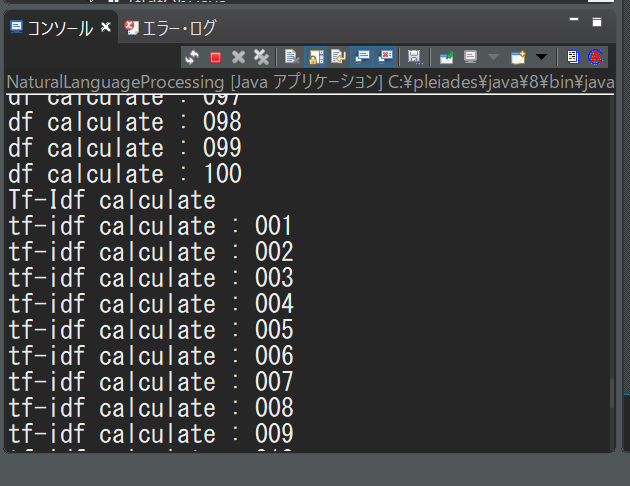
\includegraphics[scale=0.65]{tfidfstart.png}
	\caption{tfidfの計算実行時の標準出力1}
   \label{startidf}
  \end{figure}

  \begin{figure}[H]
	\centering
	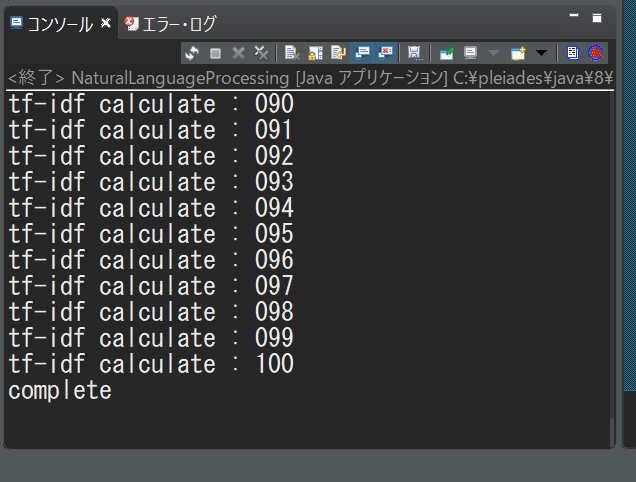
\includegraphics[scale=0.65]{tfidfend.png}
	\caption{tfidfの計算実行時の標準出力1}
   \label{endidf}
  \end{figure}

\subsubsection{tfidf値の計算結果}
リスト\ref{001tfidf}に,tfidfの計算結果を出力した001tfidf.txtの冒頭10行を示す.
リスト\ref{001tfidf}は各単語について,左から,表層系,品詞,出現回数,tf値,idf値,tfidf値の順で出力されている.
リスト\ref{001tfidf}からtfidf値は降順にソートされていることが読み取れる.
\begin{lstlisting}[basicstyle=\ttfamily\footnotesize, frame=single,label=001tfidf,caption=001tfidf.txtの冒頭10行]
天然記念物	名詞	16	0.029850746268656716	2.6989700043360187	0.0805662688
%	名詞	41	0.07649253731343283	1.013228265733755	0.0775044009
〔	記号	11	0.020522388059701493	3.0	0.0615671642
〕	記号	11	0.020522388059701493	3.0	0.0615671642
地	名詞	13	0.024253731343283583	1.6575773191777938	0.0402024350
両生類	名詞	7	0.013059701492537313	3.0	0.0391791045
生息	名詞	8	0.014925373134328358	2.3979400086720375	0.0357901494
爬虫類	名詞	7	0.013059701492537313	2.6989700043360187	0.0352477426
指定	名詞	9	0.016791044776119403	2.0969100130080562	0.0352093099
E	名詞	16	0.029850746268656716	1.013228265733755	0.0302456199
\end{lstlisting}
 tfidf値の計算結果が正しいことを確認する.ここでは「爬虫類」という単語について注目する.
リスト\ref{001tf}から「爬虫類」のtf値が0.0130597015であることが分かる.また
df.txtの出力より「爬虫類	2	名詞	2.6989700043」であるから,「爬虫類」のidf値が
2.6989700043であることが分かる.これより「爬虫類」のtfidf値は0.0352477426であることが
計算できる.リスト\ref{001tfidf}において「爬虫類」のtfidf値は0.0352477426であるから
tfidf値の計算が正しいことが確認できた.

\section{実行結果の分析と改良}
3種類の重みづけの方法について実験を行い,正しい出力ができることが確認できた.
本章では,実行結果をより細かく分析し,より良い出力結果になるようにプログラムを改良する.
ここでの,より良い出力結果とは,プログラム実行による出力結果ファイルを見たときに,
元の文書の特徴的な単語が上位に来ていることや,その文書が何について書かれているのかを読み取れる出力結果
であることを指す.例えばtfの計算結果の出力ファイルを確認したときに
「\%」,「を」を代表とするわけのわからない,もしくはどんな文書にも現れるような
単語が上位に来るのではなく,「爬虫類」,「人類」を代表とする文書の特徴を
表す単語が上位にくることが出力結果の改良にあたる.本章では次に示す実行結果の分析と改良について述べる.
\begin{enumerate}
	\item Term Frequencyの実行結果の分析
	\item Inverse Document Frequencyの実行結果の分析
	\item その他の改良点
	\item プログラムの変更点
	\item 実行結果
\end{enumerate}
\subsection{Term Frequencyの実行結果の分析}
本節ではtfの計算結果の分析として,文書の特徴を表していない語,および欠損値の除去,および品詞別のtf値について述べる.
\subsubsection{文書の特徴を表していない語}
tfの出力結果は文書1件につき,1つあるから合計で100個の出力ファイルがある.
100個のファイル全てを分析することは難しいから,ここでは001tf.txt,および002tf.txtについて
分析する.図\ref{tftop}に001tf.txt,および002tf.txtの上位の単語とそのtf値を示す.
\begin{figure}[H]
	\centering
	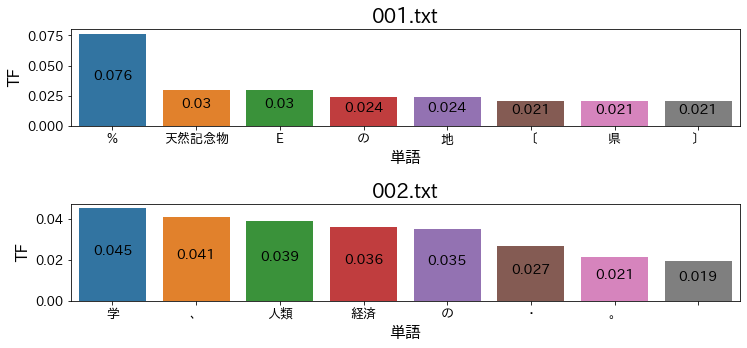
\includegraphics[scale=0.5]{tftop.png}
	\caption{001tf.txt,および002tf.txtの上位の単語とそのtf値}
   \label{tftop}
  \end{figure}

図\ref{tftop}から,tf値の高い単語として「天然記念物」,「経済」があることが読み取れる.しかし「\%」,「E」,「の」
を代表とする文書の特徴を表していない単語の方が上位に多くあることも読み取れる.「の」を代表とする助詞や,「,」は
文章中に頻繁に登場するため,tf値も多くなることが考えられる.また助詞や「,」のように文書を構成する絶対的な単語
のtf値が上位になると,本来文書の特徴を表す単語が相対的に下位になり,出力結果として埋もれてしまう.
これらの考えから,助詞を代表とするあらゆる文書に頻繁に登場する単語,および「,」を代表とする文書を構成する絶対的な
単語を形態素解析の出力結果から除外する必要があると考える.

\subsubsection{欠損値の除去}
欠損値(Missing value)とは出力結果が不正な値やデータになっている値およびデータのことである.
tfの計算結果にも標準出力にエラーとして表示されないものの,欠損値が存在する.
例えば001tf.txtの52行目の出力結果は「		名詞	2	0.0037313433」である.
この出力結果では表層系が空白(欠損値)になっている.同様の出力は002tf.txtの65行目でも
確認できる.欠損値が存在すると,001tf.txtを分析する際に上手く読み込み
が行えないことや,tfの計算結果を別のプログラムに組み込む際にエラーの原因になりかねない.このため,
tfの計算結果から,欠損値が存在する要素を排除すべきであると考える.

\subsubsection{品詞別のtf値}
助詞を代表とするあらゆる文書に頻繁に登場する単語,および「,」を代表とする文書を構成する絶対的な
単語を形態素解析の出力結果から除外する必要があると述べたが,ここではさらに品詞に着目して分析を
行う.図\ref{tfeachH}は001tf.txtおよび002tf.txtにおける品詞別のtf値の平均値である.
\begin{figure}[H]
	\centering
	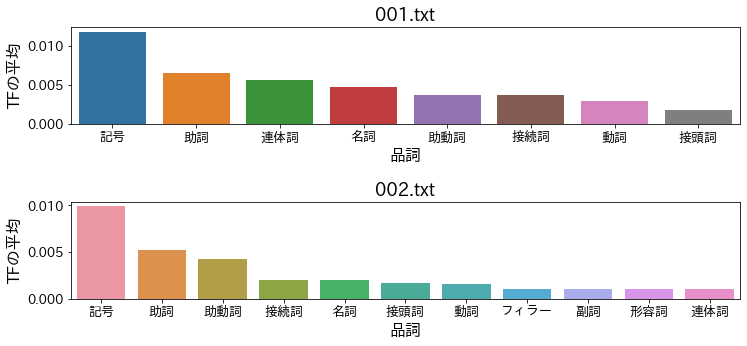
\includegraphics[scale=0.5]{tfeachH.png}
	\caption{001tf.txt,および002tf.txtの品詞別のtfの平均値}
   \label{tfeachH}
  \end{figure}

  図\ref{tfeachH}から001tf.txtでは記号,助詞,連体詞の3つのtf値の平均が高く,002tf.txtでは記号,助詞,助動詞
,接続詞の4つのtf値の平均が高いことが読み取れる.ここで,各品詞の国語的意味や役割から,
文書の特徴を表す単語になり得るかを考える.表\ref{Hinshi}に各品詞の代表例を示す.
\begin{table}[H]
	\caption{品詞の種類と代表例}
	\label{Hinshi}
	\begin{center}
		\begin{tabular}{l|l}\hline
			品詞 & 代表例 \\ \hline
			\hline
			名詞 & 東京湾,富士山,わたし,あれ,3 \\ 
			動詞 & 関わる,行う \\
			形容詞 & 面白い,青い \\ 
			形容動詞 & 立派な,便利だ \\
			副詞 & ゆっくり,とても,決して \\
			連体詞 & この,あらゆる,大きな \\
			接続詞 & だから,しかし,最初に,一方 \\
			助詞 & は,を,の \\
			助動詞 & れる,られる,ます,らしい \\ \hline
 		\end{tabular}
	\end{center}
	\end{table}

	表\ref{Hinshi}の代表例を用いて各品詞が文書の特徴を表す語か否かを考える.名詞は「東京湾」,「富士山」を代表とする
	固有名詞を含むため,文書の特徴を表す語になる.一方で「あれ」,「3」を代表とする単語は様々な文書に登場するため
	特徴を表す語にならない可能性があるため,注意が必要である.動詞は「関わる」,「行う」を代表とする動作を表す単語である.
	動作を表す単語が文書の特徴を表す単語になる可能性は低いと考える.このため動詞は形態素解析の結果から除外してよいと考える.
	形容詞,および形容動詞,および副詞は文書の特徴を表す単語としては評価難しいため今回は除外しない.連体詞は名詞を
	修飾する役割があるが,形態素解析によって文章を分割すると名詞との関係が分からなくなってしまうため除外する.
	接続詞は,前後の分を繋ぐ役割があるが,連体詞同様に形態素解析によって文章を分割すると前後の文章の関係が
	分からなくなってしまうため除外する.助詞,および助動詞は文書中に頻繁に出現する.しかし,これらの助詞,および助動詞は
	あらゆる文書に頻繁に登場するため,文書の特徴を表す語ではないと考える.よって助詞,および助動詞を除外する.

\subsection{Inverse Document Frequencyの実行結果の分析}
本節ではidfの計算結果の分析として,品詞別のdf,idfの平均値,および欠損値の除去,および文書の特徴を表していない語について述べる.
\subsubsection{品詞別のdf,idfの平均値}
図\ref{idfeachH}に品詞別のdf,およびidfの平均値を示す.
品詞別のidfの平均値を見ると,名詞,動詞,形容詞,副詞を代表とする品詞のidfの平均値にあまり差がないことが読み取れる.
このため,idfの平均値のみを見るとidfによる重み付けは品詞と関係ないことが考えられる.
また,dfの計算結果には品詞が欠損値(ここでは該当なしと表記)が存在することが読み取れる.同様に,品詞が\#になっている出力結果
が存在することも読み取れる.実験テキストの形態素IDにも品詞\#という項目は存在しない.これらの扱いについては
欠損値の除去の節で説明する.
\begin{figure}[H]
	\centering
	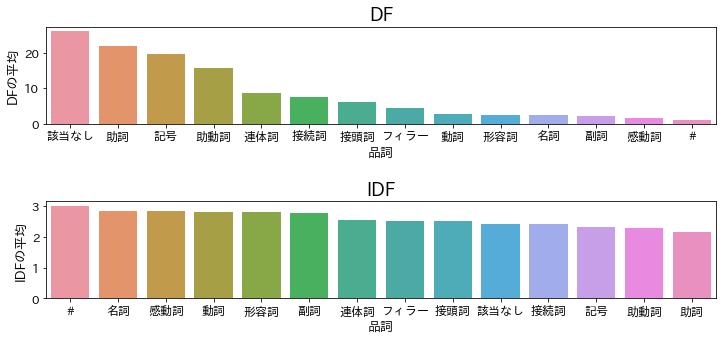
\includegraphics[scale=0.5]{idfeachH.png}
	\caption{品詞別のdfおよびidfの平均値}
   \label{idfeachH}
  \end{figure}

\subsubsection{欠損値の除去}
TermFrequencyの分析でも欠損値の除去について説明した.idfの実行結果にも欠損値が存在する.
表\ref{dfmv}にdf.txtにおける欠損値を含む行とその出力を示す.
表\ref{dfmv}から欠損値が生じている項目は単語または品詞であることが読み取れる.dfの行数17176行に対して,
欠損値が生じている単語数は5つと十分に小さいから,これらの単語は形態素解析の分析結果から除外する.
\begin{table}[H]
	\caption{df.txtの欠損値}
	\label{dfmv}
	\begin{center}
		\begin{tabular}{r|c r c c r}\hline
			行数 & 単語 & df & 品詞 & idf \\ \hline
			\hline
			12 & 欠損値 & 100 & 欠損値 & 1.00000 \\
			4060  &  )  & 2  & 欠損値 & 2.69897 \\
			9043   & .  & 1 & 欠損値 & 3.00000 \\
			10649 & " & 1 & 欠損値 & 3.00000 \\
			6956 & 欠損値 & 1 & \# & 3.0 \\ \hline
 		\end{tabular}
	\end{center}
	\end{table}

\subsubsection{文書の特徴を表していない語}
idf=1.0の単語について考える.idf=1.0の単語tのdf値は式(\ref{idf1siki})より全文書数Nであることがわかる.
$df(t) = N$ということはこの単語tは全文書に必ず登場する単語ということである.
\begin{eqnarray}
	idf(t) &=& \log_{10} \frac{N}{df(t)} +1 \\
	1  &=& \log_{10} \frac{N}{df(t)} +1 \\
	\log_{10} \frac{N}{df(t)} &=& 0 \\
	\frac{N}{df(t)} &=& 1 \\
	df(t) = N
	\label{idf1siki}
\end{eqnarray}

具体的にどのような単語が全文書に必ず登場するのか確認する.リスト\ref{idf1}にidf=1.0である単語を
列挙する.ただし,単語の区切りはカンマ(,)である.リスト\ref{idf1}から「の」,「を」を代表とする
助詞が全文書に登場したことが読み取れるが,これについては日本語の文書を構成する絶対的な
単語であるから納得できる.一方で,「出典」,「ウィキペディア」,「編集」という単語が全ての文書に
登場する.これらはwikipedia\cite{wikipedia}のページを構成する単語であると考えられる.また,これらの単語が全ての
文書に登場するということは,実験の対象にしている文書はすべてwikipediaの何らかのページで
あると考えられる.ここまでの分析は実験の対象とする文書群がウェブページ,小説,論文を代表とするあらゆる
種類の文書であるという前提で分析を行ってきたが,実験の対象としている文書群が全てwikipediaのページで
あると考えると,wikipediaのページを構成する単語は,文書の特徴にはなりえないため,
形態素解析の結果から除外して良いと考える.注意として,実験の対象とする文書群がウェブページ,小説,論文
を代表とするあらゆる種類の文書からなる場合はwikipediaのページを構成する単語も文書の特徴を
表す語になると考えられる.
\begin{lstlisting}[basicstyle=\ttfamily\footnotesize, frame=single,label=idf1,caption= idfが1.0の単語]
の, (, ), 、, 。, \\., :, は, を, に, 『, 』, ,「, 」, し, 出典, フリー,
百科, 事典, ウィキペディア, Wikipedia,移動, ナビゲーション, 検索, た, http,
://, ja, wikipedia,org, /, wiki, より, 作成, カテゴリ, \\%, E, [, ], が,
で, て, 編集, ・, 1, /%, 5, 3, 年, 8, 2
	\end{lstlisting}

\subsection{その他の改良点}
本節では次に示す4つの改良点について述べる.
\begin{enumerate}
	\item URLの除去
	\item ストップワードの除去
	\item 大文字,小文字の統一
	\item 数字の扱い
\end{enumerate}
\subsubsection{URLの除去}
実験の対象とする文書の中にはURL(Uniform Resource Locator)を含む文書が存在する.例えば付録のリスト\ref{001all}(001.txt)はURLを含む.
001.txtの形態素解析結果001.txtを見ると,URLは形態素解析によってリスト\ref{001tfurl}に示すように分解される.
形態素解析によって分解されたURLはアルファベットや数字の羅列であるから,文書の特徴を表す文書にふさわしくないと考え,除外する.
しかし,形態素解析結果から,元々URLであった単語を除外するのは難しい.そこで,元の文書から直接URLを削除する.
wikipediaのページのURLは,"「http:"で始まるから,これを文書から検出し,該当する行を削除することでURLを除外する.
\begin{lstlisting}[basicstyle=\ttfamily\footnotesize, frame=single,label=001tfurl,caption=URLの形態素解析結果の例]
/%	名詞	1	0.0018656716
94	名詞	1	0.0018656716
F	名詞	1	0.0018656716
83	名詞	1	0.0018656716
BB	名詞	1	0.0018656716
88	名詞	1	0.0018656716
AC	名詞	1	0.0018656716
99	名詞	1	0.0018656716
AB	名詞	1	0.0018656716
84	名詞	1	0.0018656716
98	名詞	1	0.0018656716
BF	名詞	1	0.0018656716
89	名詞	1	0.0018656716
80	名詞	1	0.0018656716
	\end{lstlisting}

\subsubsection{ストップワードの除去}
「機械学習のための特徴量エンジニアリング」\cite{engine}によれば,文章によらず一般的に使われる単語を特徴量(文書の特徴を表す語)に加えることは
あまり意味がない.このような単語をストップワード(stopword)と呼び,処理の対象外にするのが一般的である.
本実験ではslothlib\cite{slothlib}という日本語のストップワード辞書を利用し,形態素解析の結果からストップワードを除去する.
付録のリスト\ref{Fstop}にslothlibの日本語のストップワード辞書の抜粋を示す.
リスト\ref{Fstop}から,ストップワード辞書には,「あちら」,「あれ」を代表とする代名詞や,「年」,「月」を代表とする時間
の単位を表す単語,漢数字があることが読み取れる.\\
 また,出現頻度に基づいて文書の特徴に寄与しない単語を除去する方法もある.例えば,カナダ議会での発言を集めたHansardコーパス 
では,"House of Commons"(庶民院)という単語が頻出するため"house"という単語を文書の特徴にすべきではない.このように,通常は
有用な単語でも,特定のコーパスでは有用でない単語が存在する.このような単語を見つけ出すために頻度情報を利用する.
本実験ではdf値が90以上の単語を実験で扱うコーパスにおいて有用でないと考え,除去する.この考え方は先に述べた,
wikipedaiのページからなるコーパスからwikipediaのページを構成する単語を除外すべき,という考え方と
同じである.

\subsubsection{大文字,小文字の統一}
大文字,小文字の統一は英語の場合に有用な方法である.表\ref{OneOne}にidfの計算結果の抜粋を示す.
表\ref{OneOne}から"One"と"ONE"が実行結果に混在していることがわかる.
英語の場合,文頭の単語の頭文字を大文字にするというルールや,映画の名前によって
表記に揺れがあると考える.このような表記揺れを抑えるため,元の文書のアルファベットをすべて
小文字に置き換える処理を行う.
\begin{table}[H]
	\caption{大文字と小文字の混在}
	\label{OneOne}
	\begin{center}
		\begin{tabular}{l|c c c c}\hline
			行数 & 単語 & df値 & 品詞 & idf値 \\ \hline
			\hline 
			3016 & One & 2 & 名詞 & 2.6989700043 \\ 
			3231 & ONE & 2 & 名詞 & 2.6989700043 \\ \hline
 		\end{tabular}
	\end{center}
	\end{table}

\subsubsection{数字の扱い}
数字の扱いについて考える.数字はリスト\ref{001all}に示したように1章,2章..という章立てや,2020年,p35を代表とする
多岐にわたる部分で登場する.数字の扱いについては,章立ての場合,これは前述したwikipediaのページを構成する単語であるから
除去したい.しかし,「2020年」,「p35」を代表とする数字との区別が非常に難しい.2桁以上の数字を除去するという考え方も
あるが,章立ての多いwikipediaのページに対応できない.また,形態素解析によって「2020年」が「2020」と「年」に分解されてしまうため
数字のみを見ても単位がわからない.
実験結果の改良では出力結果の上位を見て,その文書の特徴がわかるという目標がある.出力結果の数字を見て
それが文書の特徴を表す語であると考えることは無理があると考え,本実験では数字を形態素解析の結果から除去する.
\subsection{プログラムの変更点}
分析結果から得られた改良点を次に示す.
\begin{enumerate}
	\item 記号,助動詞,助詞,接続詞,動詞,連体詞,数字の除去
	\item URLの除去
	\item ストップワードの除去
	\item 大文字,小文字の統一
\end{enumerate}

以上の改良点を実装するため,既に作成したクラスの改良および新規クラスの作成を行う.
本節では次に示すクラスの実装または追記について述べる.
\begin{enumerate}
	\item Preprocessingクラス
	\item Stopwordクラス
	\item TermFrequencyクラス
	\item NaturalLanguageProcessingクラス
\end{enumerate}

\subsubsection{Preprocessingクラス}
URLの除去および大文字,小文字の統一の統一を行うクラスとしてPreprocessingクラスを作成する.
リスト\ref{PreprocessingClass}にPreprocessingクラスのソースコードを示す.
PreprocessingクラスはフィールドにString型の配列リスト,および入出力ファイル名を持つ.
また,メソッドとして,コンストラクタ,およびpreprocessメソッド,およびcheckBeforeReadinputFileNameメソッドを持つ.
\begin{lstlisting}[basicstyle=\ttfamily\footnotesize, frame=single,label=PreprocessingClass,caption=Preprocessingクラスのソースコード]
package nlp;
import java.io.BufferedReader;
import java.io.File;
import java.io.FileNotFoundException;
import java.io.FileReader;
import java.io.FileWriter;
import java.io.IOException;
import java.util.ArrayList;

public class Preprocessing{

	ArrayList<String> list = new ArrayList<String>();
	private File inputFileName;
	private File outputFileName;
	Preprocessing(File inputFileName,File outputFileName){
		this.inputFileName = inputFileName;
		this.outputFileName = outputFileName;
	}

    public void preprocess() {
    	try{

    	      if (checkBeforeReadinputFileName(inputFileName)){
    	        BufferedReader br = new BufferedReader(new FileReader(inputFileName));

    	        String str;
    	        while((str = br.readLine()) != null){
    	          //System.out.println(str);
    	        	str = str.toLowerCase();
    	        	if (!str.contains("「http"))
      	          {
    	        		list.add(str);
      	          }

    	        }

    	        br.close();
    	      }else{
    	        System.out.println("file open error");
    	      }
    	    }catch(FileNotFoundException e){
    	      System.out.println(e);
    	    }catch(IOException e){
    	      System.out.println(e);
    	    }

    	try {
			FileWriter fw = new FileWriter(outputFileName);
			for(int i=0;i<list.size();i++) {
			fw.write(list.get(i)+"\n");
			}
			fw.close();
			list.clear();
			} catch (IOException ex) {
				ex.printStackTrace();
			 }
    }

    private static boolean checkBeforeReadinputFileName(File inputFileName){
        if (inputFileName.exists()){
          if (inputFileName.isFile() && inputFileName.canRead()){
            return true;
          }
        }

        return false;
      }
}
\end{lstlisting}

コンストラクタでは,入力ファイル名および出力ファイル名をフィールドに受け取る.
checkBeforeReadinputFileNameメソッドは引数として与えられたファイル名が存在すればtrue,存在しなければfalseを
返すメソッドである.preprocessメソッドの処理の詳細は次の通りである.
\begin{enumerate}
	\item checkBeforeReadinputFileNameメソッドを用いて入力ファイルが存在するか確認する.存在しなければ例外処理を行う.
	\item 入力ファイルを開く.
	\item 入力ファイルを1行づつ読み取り,リストに格納する.ただし,URL("「http")の文字列を含んでいる場合はリストに格納しない.また,リストに格納する際に
	toLowerCaseメソッドを用いて文字列をすべて小文字に変換する.
	\item 入力ファイルの終端までたどり着いたらファイルを閉じる.
	\item 出力ファイルを開く.出力ファイルは存在しなくても新規に作成されるため,存在するか確認する必要はない.
	\item リストの文字列を1行づつ出力する.
	\item リストの終端にたどり着いたら出力ファイルを閉じる.
\end{enumerate}

\subsubsection{Stopwordクラス}
ストップワードを読み込み,保持するクラスとして,Stopwordクラスを作成する.
リスト\ref{StopwordClass}にStopwordクラスのソースコードを示す.
StopwordクラスはフィールドとしてString型の配列リストstopwordおよび入力ファイルを持つ.
また,メソッドとしてreadStopwordメソッド,およびcheckBeforeReadinputFileNameメソッドを持つ.
\begin{lstlisting}[basicstyle=\ttfamily\footnotesize, frame=single,label=StopwordClass,caption=Stopwordクラスのソースコード]
package nlp;

import java.io.BufferedReader;
import java.io.File;
import java.io.FileNotFoundException;
import java.io.FileReader;
import java.io.IOException;
import java.util.ArrayList;

public class Stopword {
	ArrayList<String> stopword = new ArrayList<String>();
    public void readStopword(File inputFileName) {
    	try{

  	      if (checkBeforeReadinputFileName(inputFileName)){
  	        BufferedReader br = new BufferedReader(new FileReader(inputFileName));

  	        String str;
  	        while((str = br.readLine()) != null){
  	          //System.out.println(str);
  	        	str = str.toLowerCase();
  	        		stopword.add(str);
  	        }

  	        br.close();
  	      }else{
  	        System.out.println("file open error");
  	      }
  	    }catch(FileNotFoundException e){
  	      System.out.println(e);
  	    }catch(IOException e){
  	      System.out.println(e);
  	    }
    }
    private static boolean checkBeforeReadinputFileName(File inputFileName){
        if (inputFileName.exists()){
          if (inputFileName.isFile() && inputFileName.canRead()){
            return true;
          }
        }

        return false;
      }
}
\end{lstlisting}
checkBeforeReadinputFileNameメソッドの仕様はPreprocessingクラスと同様である.
readStopwordメソッドの処理の詳細は詳細は次の通りである.
\begin{enumerate}
	\item checkBeforeReadinputFileNameメソッドを用いて入力ファイルが存在するか確認する.存在しなければ例外処理を行う.
	\item 入力ファイルを開く.
	\item 入力ファイルを1行づつ読み取り,リストに格納する.
	\item 入力ファイルの終端までたどり着いたらファイルを閉じる.
\end{enumerate}

\subsubsection{TermFrequencyクラス}
TermFrequencyクラスはコーパスの形態素解析と重みづけtfを計算するクラスであった.
このクラスに記号,助動詞,助詞,接続詞,動詞,連体詞,数字,ストップワードの除去の処理を追加する.
リスト\ref{TermFrequencyClass2}にTermFrequencyクラスのソースコードの追記部分を示す.
リスト\ref{TermFrequencyClass2}のソースコードをリスト\ref{TermFrequencyClass}
の79行目に追記する.また,引数に"Stopword stopwordlist"を追加する.
追記部分の処理によって形態素解析の結果からequalsメソッドを用いて該当する品詞を検知し,リストから除外する.
また引数として受け取ったストップワードのリストに含まれる単語も形態素解析の結果から除外する.
\begin{lstlisting}[basicstyle=\ttfamily\footnotesize, frame=single,label=TermFrequencyClass2,caption=TermFrequencyクラスのソースコード(追記)]
	// 指定した品詞の語のみを抽出する

	for (int i = 0; i < list.size(); i++){
		if(list.get(i).getWord().getHinshi().equals("記号")) {
			//System.out.println(list.get(i).getWord().getHyousoukei() + "\t");
			list.remove(i);
			i--;
		}else if(list.get(i).getWord().getHinshi().equals("助動詞")) {
			list.remove(i);
			i--;
		}else if(list.get(i).getWord().getHinshi().equals("動詞")) {
			list.remove(i);
			i--;
		}else if(list.get(i).getWord().getHinshi().equals("接続詞")) {
			list.remove(i);
			i--;
		}else if(list.get(i).getWord().getHinshi().equals("助詞")){
			//System.out.println(list.get(i).getWord().getHyousoukei() + "\t");
			list.remove(i);
			i--;
		}else if(list.get(i).getWord().getHinshi().equals("連体詞")){
			list.remove(i);
			i--;
		}else if(list.get(i).getWord().getHinshi1().equals("数")){
			list.remove(i);
			i--;
		}else if(list.get(i).getWord().getHinshi().length() == 0){
			list.remove(i);
			i--;
		}
	}


	//stopwordの除外
	for (int i = 0; i < list.size(); i++){
		for(int j = 0; j<stopwordlist.stopword.size();j++) {
			if(list.get(i).getWord().getHyousoukei().equals(stopwordlist.stopword.get(j))) {
				list.remove(i);
				i--;
				break;
			}
		}
	}
\end{lstlisting}

\subsubsection{NaturalLanguageProcessingクラス(メイン)}
メインクラスに,コーパスの下処理を追記する.
リスト\ref{NaturalLanguageProcessingClass4}にNaturalLanguageProcessingクラスのソースコードを示す.
ただし,idfおよびtf-idfの計算を行うプログラムは既に示しているから,省略する.
追記部分である10行目から18行目では100件のファイルについてPreprocessingクラスをインスタンス化し,下処理を行っている.
また,19行目から22行目でストップワードの読み込みを行い,32行目でtfメソッドの引数としてオーバーライドしたtfメソッドを実行している.
\begin{lstlisting}[basicstyle=\ttfamily\footnotesize, frame=single,label=NaturalLanguageProcessingClass4,caption=NaturalLanguageProcessingクラスのソースコード(追記)]
package nlp;

import java.io.File;

public class NaturalLanguageProcessing
{
 static public void main(String args[])
 {

 System.out.println("Preprocessing");
 System.out.println("deleteURL");
 for(int i=1; i<=100;i++) {
	 File inputFileName = new File("data-utf8\\" + String.format("%03d", i) + ".txt");
	 File outputFileName = new File("data-utf8\\" + String.format("%03d", i) 
	 + "changed.txt");
	 System.out.println("data-utf8\\" + String.format("%03d", i) + "changed.txt");
	 Preprocessing pre = new Preprocessing(inputFileName,outputFileName);
	 pre.preprocess();
 }
 System.out.println("readstopword");
 File stopwordName = new File("data-utf8\\stopword.txt");
 Stopword stopwordlist = new Stopword();
 stopwordlist.readStopword(stopwordName);

 System.out.println("TF calculate");
 TermFrequency[] tf= new TermFrequency[100];
 for(int i=1; i <= 100;i++){
	 tf[i-1] = new TermFrequency();
	 String inputFileName = "data-utf8\\" + String.format("%03d", i) + "changed.txt";
	 String outputFileName = "data-utf8\\" + String.format("%03d", i) + "tfchanged.txt";
	 //System.out.println(inputFileName);
	 System.out.println(outputFileName);
	 tf[i-1].tf(inputFileName,outputFileName,stopwordlist);
	 //tf[i-1].tf(inputFileName,outputFileName);
 }

// idfおよびtf-idfのプログラムは省略
 }
}

\end{lstlisting}

\subsection{実行結果}
実行結果として,ファイル出力を確認する.
リスト\ref{001tfidfk}に001tfidf.txtの冒頭10行を示す.また,リスト\ref{002tfidfk}に002tfidf.txtの冒頭10行を示す.
リスト\ref{001tfidfk}およびリスト\ref{002tfidfk}から,どちらの出力結果においても,リスト\ref{001tf}やリスト\ref{002tf}
のように「\%」を代表とする記号,「の」,「を」を代表とする助詞といった文書の特徴を表していない語が上位に
ない.また,「天然記念物」,「両生類」,「経済」を代表とする文書の特徴を表す語が上位にあることが読み取れる.
\begin{lstlisting}[basicstyle=\ttfamily\footnotesize, frame=single,label=001tfidfk,caption=001tfidf.txtの出力内容(改良後)]
天然記念物	名詞	16	0.0851063829787234	2.6989700043360187	0.2296995748
両生類	名詞	7	0.03723404255319149	3.0	0.1117021277
生息	名詞	8	0.0425531914893617	2.3979400086720375	0.1020400004
爬虫類	名詞	7	0.03723404255319149	2.6989700043360187	0.1004935640
指定	名詞	9	0.047872340425531915	2.0969100130080562	0.1003839900
オオサンショウウオ	名詞	5	0.026595744680851064	3.0	0.0797872340
カジカガエル	名詞	3	0.015957446808510637	3.0	0.0478723404
ウミガメ	名詞	3	0.015957446808510637	3.0	0.0478723404
特別	名詞	4	0.02127659574468085	2.221848749616356	0.0472733777
繁殖	名詞	3	0.015957446808510637	2.5228787452803374	0.0402587034
	\end{lstlisting}

\begin{lstlisting}[basicstyle=\ttfamily\footnotesize, frame=single,label=002tfidfk,caption=002tfidf.txtの出力内容(改良後)]
人類	名詞	38	0.080338266384778	2.5228787452803374	0.2026837047
経済	名詞	35	0.07399577167019028	2.3979400086720375	0.1774374214
学	名詞	44	0.09302325581395349	1.7958800173440752	0.1670586063
訳	名詞	11	0.023255813953488372	2.221848749616356	0.0516709012
社会	名詞	13	0.02748414376321353	1.7695510786217261	0.0486345962
文化	名詞	10	0.021141649048625793	1.7695510786217261	0.0374112279
市場	名詞	6	0.012684989429175475	2.3010299956639813	0.0291885412
ポランニー	名詞	4	0.008456659619450317	3.0	0.0253699789
栗本	名詞	4	0.008456659619450317	3.0	0.0253699789
慎一郎	名詞	4	0.008456659619450317	3.0	0.0253699789
			\end{lstlisting}

\section{考察}
本章では,プログラム改良後の分析,および実験全体の考察について述べる.
\subsection{プログラム改良後の分析}
プログラム改良後の出力結果を分析し,改良の効果について考察する.
単語の除去によってどの程度の単語が除外されたのかを調べる.文書の特徴を表さない単語のtf値を代表とする重みづけを計算する
時間は無駄であるから,定量的に除外された単語の個数を調べることで,どの程度無駄な処理が削減されたかが分かる.
表\ref{describe-word}に改良前および改良後における,文書100件の単語の分布の統計量を示す.
また,図\ref{boxplot}に改良前および改良後における,文書100件の単語の分布の箱ひげ図を示す.
表\ref{describe-word}および図\ref{boxplot}から,改良前の単語数の分布では平均値が450単語付近,中央値が400単語付近であることが読み取れる.
一方で改良後の単語数の分布は平均が300単語付近であるから,単語数全体の傾向として,改良前より平均150単語程度減少していることが分かる.
また,改良前は外れ値が6つ存在するが,改良後は外れ値が3つになっている.

\begin{table}[H]
	\caption{改良前および改良後の単語数の分布の統計量}
	\label{describe-word}
	\begin{center}
		\begin{tabular}{l|r r}\hline
			統計量 & 改良前 & 改良後 \\ \hline
			\hline	
			平均 & 452.60 & 305.950	\\
			標準偏差 & 232.600624 & 190.211917	\\
			最小値 & 131.00	& 57.00	\\
			第一四分位数 & 294.500 & 176.7500	\\
			中央値(第二四分位数) & 394.00 & 251.500	\\
			第三四分位数 & 533.00 & 398.500	\\
			最大値 & 1323.00 & 1009.00	\\ \hline
 		\end{tabular}
	\end{center}
	\end{table}

\begin{figure}[H]
	\centering
	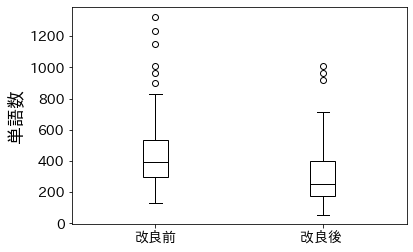
\includegraphics[scale=0.75]{boxplot.png}
	\caption{改良前と改良後の単語数の分布}
   \label{boxplot}
  \end{figure}

改良前の文書の単語数を1としたときの,改良後の文書の単語の割合から,どの程度の単語が除外されたかを確認する.
図\ref{histgram}に改良前の単語数を1としたときの改良後の単語数のヒストグラムを示す.
図\ref{histgram}から改良後の単語数は,改良前の単語数のおおよそ55\%から70\%になっていることが
読み取れる.これより改良前の単語の30\%から45\%は文書の特徴を表さない意味のない単語であることが
わかる.30\%から45\%の単語を除外することによって得られる処理時間の高速化は非常に大きいと考える.
\begin{figure}[H]
	\centering
	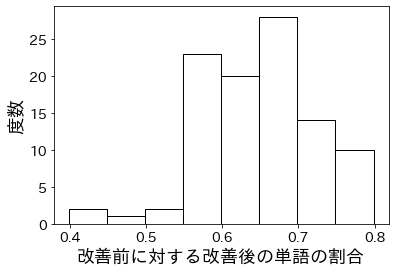
\includegraphics[scale=0.75]{histgram.png}
	\caption{改良前に対する改良語の単語の割合}
   \label{histgram}
  \end{figure}

しかし,改良後も文書の特徴を表さない単語が完全になくなったわけではない.
リスト\ref{dfchanged}に改良後のdf.txtの冒頭15行を示す.
リスト\ref{dfchanged}から「-」,「.」,「(」を代表とする記号
が残っていることが読み取れる.記号は除外するように改良したはずである.
これらの記号が残っている理由は品詞が名詞になっているためであると考える.
冒頭15行以外にも記号が残っているが,df.txtは14191単語あるため,
これらをひとつずつ確認して除外する作業は困難であると考える.
\begin{lstlisting}[basicstyle=\ttfamily\footnotesize, frame=single,label=dfchanged,caption=df.txtの出力内容(改良後)]
-	名詞	82	1.0861861476
関連	名詞	75	1.1249387366
非	接頭詞	75	1.1249387366
項目	名詞	72	1.1426675036
目次	名詞	72	1.1426675036
表示	名詞	72	1.1426675036
.	名詞	67	1.1739251973
日本	名詞	65	1.1870866434
(	名詞	59	1.2291479884
)	名詞	55	1.2596373105
/	名詞	54	1.2676062402
リンク	名詞	52	1.2839966564
外部	名詞	49	1.3098039200
現在	名詞	45	1.3467874862
編	名詞	42	1.3767507096
\end{lstlisting}

\subsection{実験全体の考察}
形態素解析,Term Frequency,Inverse Document Frequency,tf-idfの実装を通して,自然言語処理における言語処理の基礎的な知識および開発環境を学ぶ
という目的を達成できたと考える.
また,結果を分析し文書の特徴を抽出するように改良を行うという目的は主観的ではあるが達成できたと考える.
客観的に文書の特徴を表す語が抽出できているかを判断する方法としては,Tf-Idfによる重みづけを利用し,
2つの文書の類似度を測る方法(コサイン類似度)が存在する.この方法では文書の特徴を表す語が
抽出できているか否かが,2文書間の類似度の数値に大きく影響を表すため,文書の特徴を抽出するように改良を行う
という目的を評価するよい指標になると考える.

\section{付録}
本章では付録として001.txtの内容全文,およびストップワード辞書の内容の抜粋について述べる.
\subsection{001.txtの内容全文}
リスト\ref{001all}に001.txtの全文を示す.
\begin{lstlisting}[basicstyle=\ttfamily\footnotesize, frame=single,label=001all,caption=001.txtの全文]
両生類・爬虫類天然記念物一覧
出典: フリー百科事典『ウィキペディア(Wikipedia)』
移動: ナビゲーション, 検索 
両生類・爬虫類天然記念物一覧は、日本の文部科学大臣が指定する、天然記念物(特別
天然記念物を含む、以下同)のうち、両生類・爬虫類に関わるもののリスト。天然記念
物指定基準「動物」に基づき指定されたもののうち、両生類・爬虫類の種および生息地、
繁殖地等を掲載する。なお、本項では文化財保護法に基づき国(日本国文部科学大臣)
が指定した天然記念物を対象とし、地方自治体指定の天然記念物は対象外とする。

目次 [非表示]
1 特別天然記念物
2 天然記念物 
2.1 両生類
2.2 爬虫類
3 関連項目
4 参考文献
5 外部リンク
 
 特別天然記念物 [編集]
オオサンショウウオ(種指定)
 天然記念物 [編集]
 両生類 [編集]
(オオサンショウウオ) 
オオサンショウウオ生息地〔岐阜県郡上市和良町・八幡町〕
オオサンショウウオ生息地〔岐阜県郡上市大和町〕
オオサンショウウオ生息地〔岡山県真庭市〕
オオサンショウウオ生息地〔大分県宇佐市〕
(カジカガエル) 
湯原カジカガエル生息地〔岡山県真庭市〕
南桑カジカガエル生息地〔山口県岩国市〕
(モリアオガエル) 
大揚沼のモリアオガエルおよびその繁殖地〔岩手県八幡平市〕
平伏沼モリアオガエル繁殖地〔福島県双葉郡川内村〕
 爬虫類 [編集]
(アオダイショウ) 
岩国のシロヘビ
(アカウミガメ) 
御前崎のウミガメおよびその産卵地〔静岡県御前崎市〕
大浜海岸のウミガメおよびその産卵地〔徳島県海部郡美波町〕
キシノウエトカゲ
(クサガメ) 
見島のカメ生息地〔山口県萩市〕
セマルハコガメ
リュウキュウヤマガメ
 関連項目 [編集]
天然記念物
レッドリスト
 参考文献 [編集]
加藤睦奥雄ら監修 『日本の天然記念物』 講談社、1995年、ISBN 4-06-180589-4。
 外部リンク [編集]
文化庁 
国指定文化財等データベース
国宝及び重要文化財指定基準並びに特別史跡名勝天然記念物及び史跡名勝天然記念物指定基準
「http://ja.wikipedia.org/wiki/%E4%B8%A1%E7%94%9F%E9%A1%9E%E3%83%BB%E7%88%AC
%E8%99%AB%E9%A1%9E%E5%A4%A9%E7%84%B6%E8%A8%98%E5%BF%B5%E7%89%A9%E4%B8%80%E8%
A6%A7」より作成
カテゴリ: 両生類・爬虫類天然記念物 | 動物関連の一覧
	\end{lstlisting}

\subsection{ストップワード辞書の内容の抜粋}
リスト\ref{Fstop}にストップワード辞書の抜粋を示す.
\begin{lstlisting}[basicstyle=\ttfamily\footnotesize, frame=single,label=Fstop,caption=ストップワード辞書の抜粋]
あそこ,あたり,あちら,あっち,あと,あな,あなた,あれ,いくつ ...
(中略)
上,中,下,字,年,月,日,時,分,秒,週,火,水,木,金,土,国,都,道,府,県,市,区,町,村...
(中略)
春,夏,秋,冬,一,二,三,四,五,六,七,八,九,十,百,千,万,億,兆,下記,上記,時間,今回,
前回,場合,一つ,年生,自分,ヶ所,ヵ所,カ所,箇所,ヶ月...
(後略)
	\end{lstlisting}


\begin{thebibliography}{9}
	\bibitem{mecab} MeCab,\url{https://taku910.github.io/mecab/} ,閲覧日2020年7月12日
	\bibitem{javaapi} Java(tm) Platform Standard Edition 8 API,\url{https://docs.oracle.com/javase/jp/8/docs/api/} ,閲覧日2020年7月12日
	\bibitem{wikipedia} wikipedia,\url{https://ja.wikipedia.org/wiki/%E3%83%A1%E3%82%A4%E3%83%B3%E3%83%9A%E3%83%BC%E3%82%B8} ,閲覧日2020年7月12日
	\bibitem{engine} Alice Zheng・Amanda Casari,"機械学習のための特徴量エンジニアリング",株式会社オーム社,2019
	\bibitem{slothlib} slothlib,\url{http://svn.sourceforge.jp/svnroot/slothlib/CSharp/Version1/SlothLib/NLP/Filter/StopWord/word/Japanese.txt} ,閲覧日2020年7月12日

\end{thebibliography}
\end{document}
